% This template was created by Ben Mitchell
% for Dr. Sheppard's AI class, CS 335/435, spring 08.

% For those who want to learn LaTeX, this is a decent place to start:
% http://en.wikibooks.org/wiki/LaTeX
% Note that the proper pronunciation is "la tek", not "lay teks".
%
% There are lots of latex tutorials and primers online; just be careful with
% google images.

\documentclass[12pt,letterpaper]{article}

\usepackage{amsmath, amsthm, graphicx, multicol}

\title{AI Learning Polar Tic-Tac-Toe: \\ Simple Hurestic, Naive Bayes, Temporal Difference Neural Network, Minimax}
\author{Jacob Barthelmeh, Kaleb Himes, Angelica Davis}

\begin{document}
\maketitle

\begin{abstract}
This is an experiment to compare the ability of four different algorithms to win a polar tic tac toe game. The four algorithms used are; a simple heuristic, Naive Bayes Network, Temporal Difference Neural Network (TDNN) and the Minimax Algorithm. Algorithms are compared in their ability to learn and their ability to win when compared.
\end{abstract}

\section{Introduction}
In the first section of your paper, which should be entitled ``Introduction,''
you should introduce the subject of your paper to the reader.  There are several
components to this.  You probably want to begin by talking about what problem
your work is trying to solve, and why it is a problem worth trying to solve.
Explain to your reader why they should care.  This is also a good time to
introduce basic nomenclature related to your subject.  You can assume that your
reader is a reasonably well educated individual and has some knowledge of
computer science, but you should not assume that they are an expert in your field.  You have
spent a bunch of time studying your topic (in this case, game AI), but
your reader may not have.  Take the time to bring him or her up to speed; this
is what the introduction is all about.

The introduction in a real paper is generally several pages, but yours does not
need to be that long for this assignment.  It should, however, be long enough to
convey the information you need to convey.  It should move from the initial, high level
overview of the topic to a more detailed description of what other related work
has been done on the topic, and any other background information needed to
understand the later parts of the paper.  For example, you should talk about the nature
of game search in general, and what other work has been
done to solve this important problem.  More specific details of the algorithms and
techniques you used should wait for later sections.

Because your introduction discusses prior related work, you should be sure to
properly cite that prior related work. An example citation is included here \cite{tesauro1995temporal}.
If your introduction does not have at
least a couple of citations, then it is either inadequate in scope, or it fails
to properly cite works referenced.  Later sections of the
paper should also contain proper citations where needed, but the bulk of the
citations in any given paper can usually be found in the introduction or a 
separate related works section, as that
is where the most related publications are discussed.

Your introduction should conclude by describing the organization of the rest of
the paper; for example:
\begin{quote}
`` a’’
\end{quote}

Not all papers have this sort of organizational statement, but it can be helpful
due to the fact that the naming and organization of the sections in papers are
not entirely standard.  While almost all scientific papers begin with an
introduction, then discuss the experiments and results, and finally conclude,
the precise organization of that middle part can vary somewhat based on the
subject matter and the preferences of the author (or sometimes the journal).





The TDNN uses gradient descent when training \cite{gradientTDNN}.
\cite{stanfordTDNN}
\cite{robotTDNN}


\section{Problem Statement}
Algorithms will be used to play Polar Tic-Tac-Toe. The game is played by alternating turns of who gets to pick a move on the board. Spots picked are represented visually by a O or an X indicating which player has chosen the spot .  {\hl}[red]......continue explaining{\rule}

How the algorithms interact with the game is that the current board state is passed to them at any given time. The algorithm than takes the representation of the board and determines what it's next move would be. Once having done this it returns a representation of the new board state that then gets rendered by the GUI.

\subsection{Traditional Minimax Search}
Here, talk about minimax search in game playing.  You can give the generic
algorithm for minimax, and talk about the the conditions under which minimax
is appropriate.

\subsection{Minimax with Alpha-Beta Pruning}
Here, talk about how the alpha-beta algorithm works.  Give the basic algorithm, and
discuss what needs to be done for your implementation.

\subsection{Heuristic Functions}
Here you discuss the heuristic functions that have been developed to assist the
game playing agent. You need to provide a formal specification of the algorithm
in as much mathematical detail as possible. The following is an example using
the equation editing capabilities of \LaTeX{} to illustrate using this powerful capability.
\[
V^\pi(s)=\max_{a in \mathcal{A}} \left[ R(s,a) + \gamma \sum_{s' \in \mathcal{S}} P(s'|s,a) V(s') \right].
\]

\subsection{Win Checking with Resolution}
In this section, you will describe your win checker and how you specified your rules. 
You should include the rules if there are not too many of them. Otherwise, list the most important
ones (but be sure to include all of the rules in your design document). You also need to describe 
your unification procedure and your resolution procedure. This is not the place to include code; 
however, you may provide pseudocode if you think it will help the description.

\subsection{Game Evaluation with Classifiers}
This is where the description of your classifier is included. You need to explain what kind of
classifier you used, how it works, and how you trained it.

\subsection{Temproal Diffrence Neural Network}
\begin{quote}
`` 
In some respects, this is the most important section of the paper since it details how
you implemented the reinforcement learning. Here, you describe the algorithm, the
neural network, and the training process.
’’
\end{quote}



When training the TDNN the first 20 games are trained against a random player. This is in hopes of rudecing the risk of falling into an early local minumum. The remander of n games chosen to be trained by a user is than done by pitting the current TDNN against itself. After each game is played the final result is evaluated and each state leading up to the result is compared to the perdiction given by the network. Gradient descent is than done using the error of the network and allowing for adjustments to be made to the networks weights. For each game the network is trained for both players, having the weights adjusted from both players perspectives after each game has ended.

\section{Experimental Methods}
\begin{quote}
`` 
In this section, you describe your experimental methodology; this is where you talk
about your data and what you did with it.  Talk about what sorts of experiments
you performed, and how you validated them.  For example, if you used self-play
or you experimented with a human playing with the computer, you would say that 
you used it, define what it is, and discuss how you implemented it.  

Since this project includes several requirements to be satisfied, this is where you describe
how those requirements are tested, and how the resulting features are being compared.
A well constructed experiment (and your description of that experiment) will go a long
way towards demonstrating that you met the project's requirements.
’’
\end{quote}

\section{Results}
\begin{figure}
\begin{center}
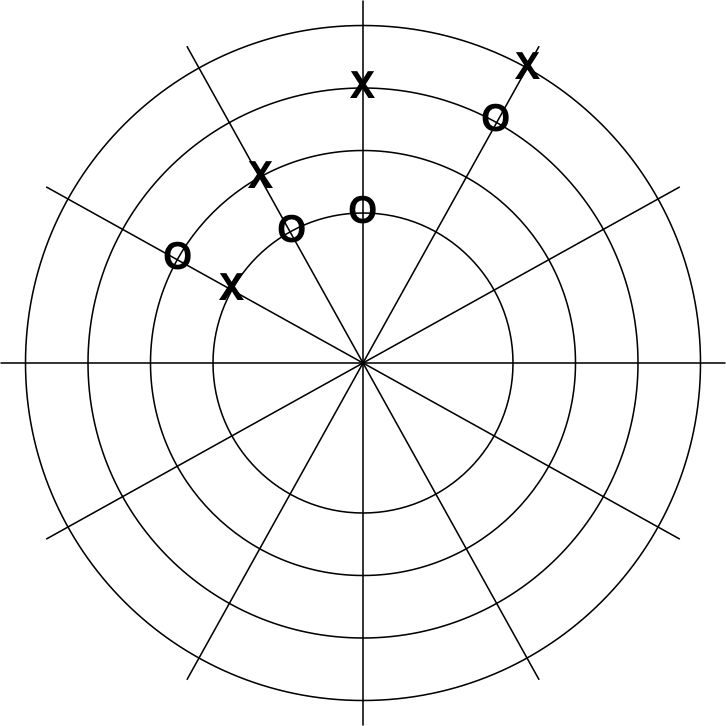
\includegraphics[width=2.5in]{P-TTT-ex.png}
\end{center}
\caption{This is a caption on the figure}
\label{somefigure}
\end{figure}

\begin{table}
\begin{center}
\begin{tabular}{|c||c|c|c|}
\hline
& col1 & col2 & col3\\
\hline \hline
row1 & a & b & c\\
\hline 
row2 & d & e & f\\
\hline 
\end{tabular}
\end{center}
\caption{This is a caption on the table}
\label{sometable}
\end{table}

The results section should contain your results.  It should \emph{not} contain
your interpretation of those results.  That comes later.  This section should be
made up primarily of graphs and tables that show your data.  You should also
have a small amount of text describing what each of the tables and graphs shows,
since the caption on the figures should be short.  Having text describing the
specifics of the experiment that led to that particular table would also be
good.  

I am not going to tell you exactly what tables or graphs you should have here,
since it will depend a bit on your results.  You should be sure that your
results section contains sufficient data to support your conclusions about the
relative strengths and weaknesses of the different algorithms.  You should also
be sure that your data is complete; that is, do not leave data out simply because
it does not support the point you are trying to make.

You should also be sure that your results are clear and interpretable.  Seven
pages of raw binary data will do nothing to edify your reader.  Similarly, a
1 inch square graph with 12 lines plotted on it will be difficult to extract
meaning from, as will a graph with poor (or no) labels on the axes.  Your
results should be legible both on screen and in hard copy. By the way, do
not rely on color difference to make your points since many people read
black-and-white print outs of the papers (including your instructor).

You do not want to present results that are just raw data, since that is hard to
interpret.  But you do not want to be overly abstract, either, since that leads to
results that have little or no meaning (e.g., ``the average over all different
data sets, algorithms, and parameters'' is a completely useless statistic for
comparing algorithms).

\section{Discussion}
The discussion section is where you discuss your interpretation of the data you
presented in the results section.  This is where you tell the reader how great
your algorithm is, and how interesting it is that \emph{this} performed better
than \emph{that} on some given data set.  You can also speculate about causes
for interesting behaviors; for example, if you think you might know why it fails
so badly on some particular case, or if you have an insight into why it did well
on another case.  You do not want to be making wild guesses, but as long as you
make it clear that you are not making claims of factual proof, you can go out on
a limb a little.  For example,

\begin{quote}
``In most cases, algorithm A outperforms algorithm B with a significance of
99.8\%.  However, as can be seen from Figure \ref{somefigure}, when applied to
the E. E. Smith data set, algorithm A does no better than random chance.  It
seems likely that the failure of algorithm A to learn is due to the extremely
sparse distribution of that data set.  Because of algorithm A's heavy reliance
on data being densely sampled from the true underlying distribution, any sparse
data set is likely to show this behavior.''
\end{quote}

\section{Conclusions}
The conclusion section should be relatively short, and should not be a summary
of your paper.  It should, however, bring up what you learned and what impact
your results have on the rest of the field (and society as a
whole, if applicable).  You should conclude, and bring your paper to an  end
with any parting thoughts that are appropriate.

Certain types of papers can be ended with a ``Summary'' section instead of a
``Conclusions'' section, in which case you would, in fact, summarize the main
points of your paper.  For this paper, you should write a Conclusions section,
not a Summary.

Conclusions also often contain information about what else you would like
to do.  Sometimes this is a separate subsection, or even a section, entitled
``Future Work.''  The basic idea here is to talk about what the next steps to
take would be.  This is of benefit to others who are interested in your
work and may want to help advance it.  It is also a chance for you to
acknowledge shortcomings in your work; since we never have infinite time to
prepare a paper, there are always more experiments that would have been nice to
include.  If you list them as future work, then it at least makes it clear that
you did not do those things because you didn't have time, rather than because you
didn't realize that they were important to do.

In your paper, you should include a brief discussion of avenues for possible
future work in your Conclusions section.  It should be tied in with the rest of
your conclusion, and should not be an unrelated section tacked on the end (or
the middle).

\bibliographystyle{plain}
\bibliography{refrences}

\end{document}
